\documentclass{beamer}
%%%%%%%%%%%%%%%%%%%%%%%%%%%%%%%  Packages  %%%%%%%%%%%%%
\usepackage{amsmath} 
\usepackage{mathtools}
\usepackage{physics}
\usepackage{amssymb}
\usepackage{mathptmx}
\usepackage{array}
  
%%%%%%%%% FIGurES %%%%%%%%%%%%%%%%%%%%%%%%
\usepackage{textcomp}
\usepackage{graphicx}
\usepackage{caption} 
\usepackage{subcaption}
\usepackage{scrextend}
\usepackage{rotating}
\usepackage{float}
\usepackage{url}
\usepackage{hyperref}
\graphicspath{{../figures/}}
\hypersetup{colorlinks=true, citecolor=blue, linkcolor=blue}
\renewcommand{\equationautorefname}{Eq.}
\renewcommand{\figureautorefname}{Fig.}
 
%%%%%%%%%%%% LaNgUaGe %%%%%%%%%%%%%%%%%%
\usepackage{verbatim}
\usepackage{natbib}
%\usepackage{qcircuit}
\usepackage{wrapfig}

\usepackage[utf8]{inputenc}
\usetheme{PaloAlto}

\title{Cohort Project update}
\author{Cohort 4}
\institute{Quantum Engineering CDT \\ University of Bristol}
\date{\today}

% plan

\begin{document}

\frame{\titlepage}

% slide 1
\begin{frame}
\frametitle{Survey results}
\begin{figure}[H]
	\centering
	
\includegraphics[width=0.5\textwidth]{survey.pdf}
	\caption{Results from onedrive \url{link}}
	\label{}
\end{figure}
\end{frame}

% slide 1
\begin{frame}
\frametitle{Sections we plan to include}
\begin{figure}[H]
	\centering
	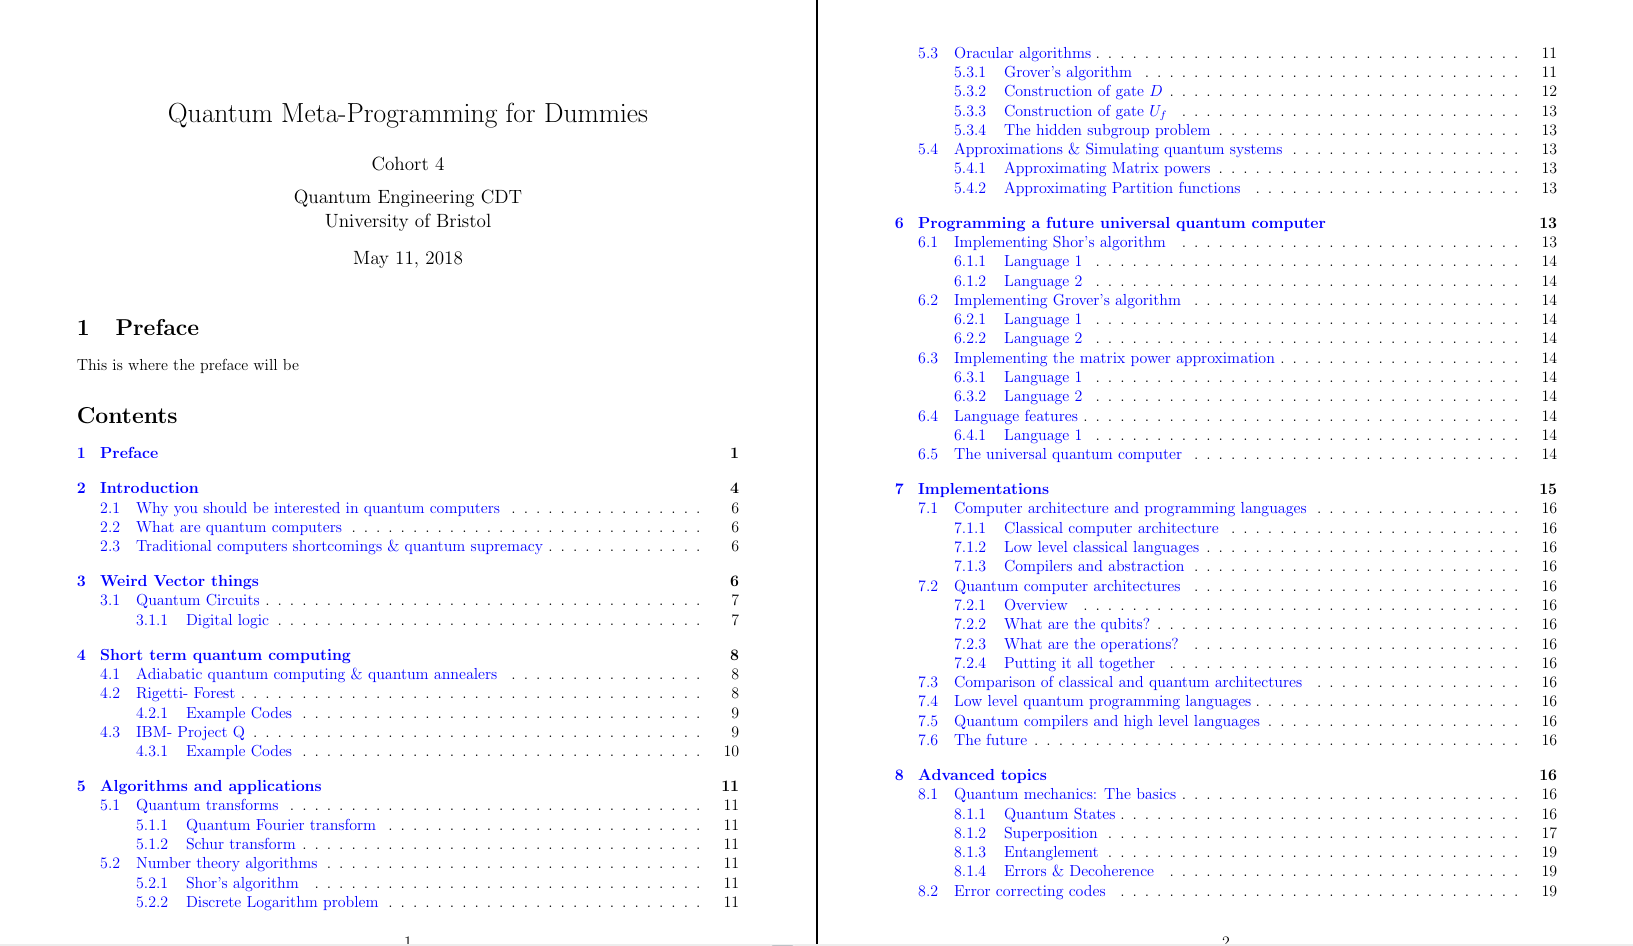
\includegraphics[width=0.95\textwidth]{cohortprojcontents.png}
	\caption{Document at \url{https://github.com/ot561/qprogramming/blob/master/main.pdf}}
	\label{}
\end{figure}
\end{frame}


\end{document}

